\documentclass[10pt,handout]{beamer}
%\documentclass[10pt]{beamer}
\usepackage[english]{babel} % Anpassa efter svenska. Ger svensk logga.
\usepackage[utf8]{inputenc} % Anpassa efter linux
\usepackage{graphicx}
\usepackage{hyperref}

\hypersetup{
    colorlinks=true,
    linkcolor=blue,
    filecolor=magenta,
    urlcolor=cyan,
}

\usetheme{Uppsala}
%\usecolortheme{UU} % Anpassa efter UU:s frger och logga
%\hypersetup{pdfpagemode=FullScreen} % Adobe Reader ska ppna fullskrm
\setbeamertemplate{itemize items}[circle]

% \usepackage{beamerthemesplit}
\usepackage{amsmath}
% \usepackage{amssymb}
% \usepackage{graphics}
% \usepackage{graphicx}
% \usepackage{epsfig}
% \usepackage[latin1]{inputenc}
 \usepackage{color}
% \usepackage{fancybox}
% \usepackage{psfrag}
% \usepackage[english]{babel}
 \setbeamertemplate{footline}{\hfill\insertframenumber/\inserttotalframenumber}

%\usepackage{bm}
%\usepackage{natbib}
\newcommand{\bfm}[1]   {\mbox{\boldmath{${#1}$}}}
\newcommand{\Prob}   {\mbox{\textnormal{P}}}
\def\eqd{\,{\buildrel d \over =}\,}

%%%%%%%%%%%%%%%%%%%%%%%%%%%%%%%%%%%%%%%%%%%%%%%%%%%%%%%%%%%%%%%%%%

\setlength{\parskip}{3mm}
\title[]{{\color{black}Machine learning, big data and artificial intelligence -- Block 1}}
\author[]{M{\aa}ns Magnusson\\Department of Statistics, Uppsala University}
\date{November 2020}


\begin{document}

\frame{\titlepage
% \thispagestyle{empty}
}

%%%%%%%%%%%%%%%%%%%%%%%%%%%%%%%%%%%%%%%%%%%%%%%%%%%%%%%%%%%%%%%%%%


\begin{frame}{This week's lectures}
\begin{itemize}
\item What is AI and Machine Learning?
\item Course Information and Practicalities
\item Introduction to Supervised Learning
\item (Stochastic) Gradient Descent
\end{itemize}
\end{frame}

\section{What is AI and ML?}
\frame{\sectionpage}

\begin{frame}{What exactly is machine learning and artificial intelligence?}
The word "AI" is often used quite loosely:
   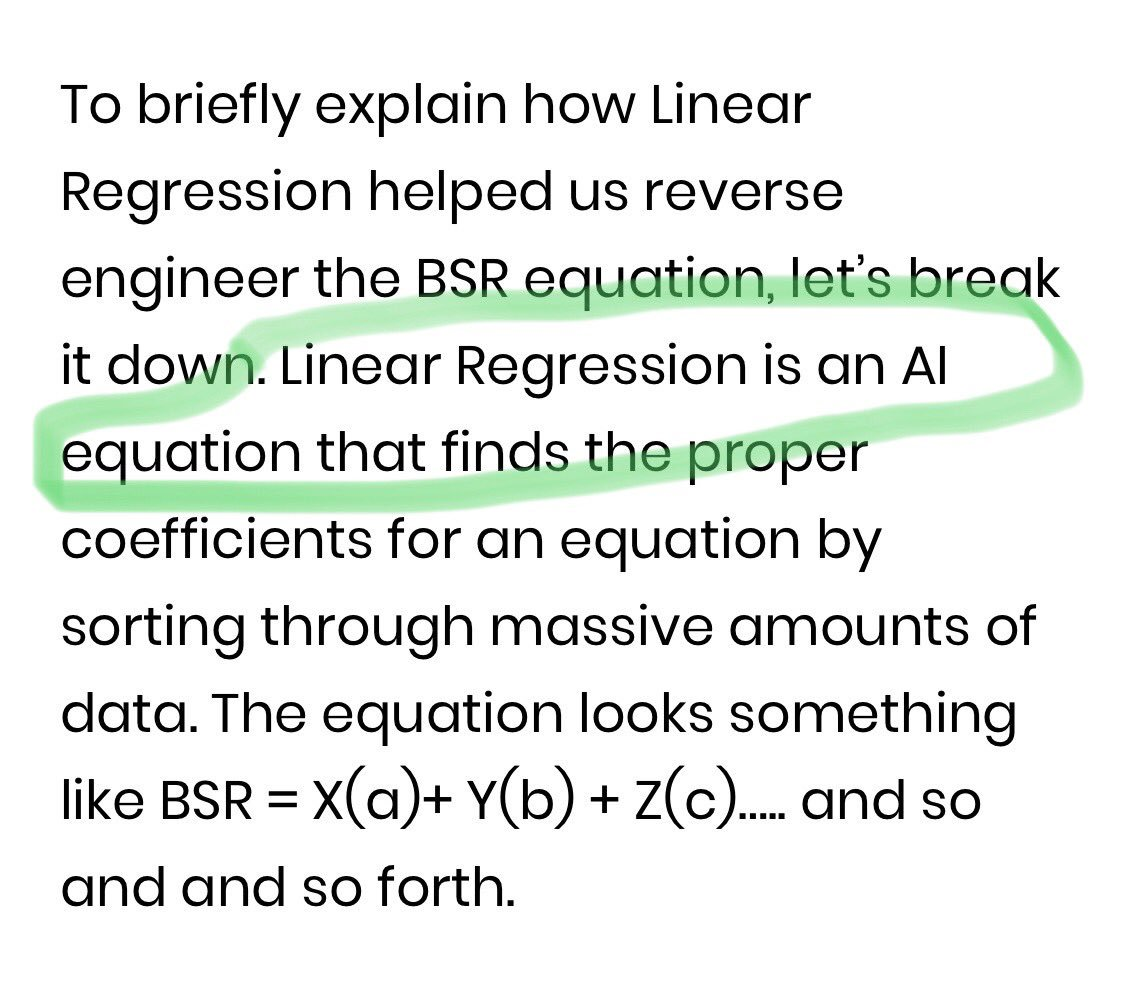
\includegraphics[width=\textwidth]{figs/AI-example.jpg}
\end{frame}


\begin{frame}{What is Artificial Intelligence?}
Artificial intelligence (AI), sometimes called machine intelligence, is intelligence demonstrated by machines, unlike the natural intelligence displayed by humans and animals. -- Wikipedia

Artificial intelligence (AI), the ability of a digital computer or computer-controlled robot to perform tasks commonly associated with intelligent beings. -- Encyclopedia Brittanica
\end{frame}


\begin{frame}{What is Artificial General Intelligence?}

Artificial general intelligence (AGI) is the hypothetical intelligence of a machine that has the capacity to understand or learn any intellectual task that a human being can. -- Wikipedia

Also called:
\begin{enumerate}
\item Strong AI
\item General AI
\item Full AI
\end{enumerate}

\end{frame}



\begin{frame}{What is Machine Learning?}

Machine Learning is the field of study that gives the computer the ability to learn without being explicitly programmed. -- Arthur Samuel (1959)

A computer program is said to learn from experience E with respect to some class of tasks T and performance measure P, if its performance at tasks in T, as measured by P, improves with experience E. -- Tom Mitchell (1998)\pause

Learning from data. -- Hastie, Tibshirani, Friedman (2009)
\end{frame}


\begin{frame}{What is Machine Learning?}

\begin{figure}[h]
\caption{ML, AI and DL (Chollet, 2018, Figure 1.1)}
\centering
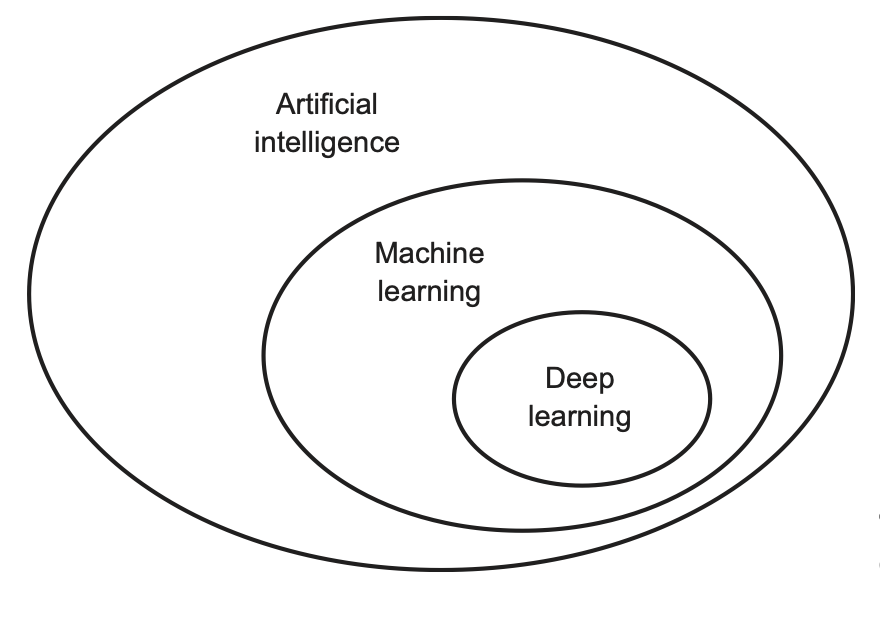
\includegraphics[width=0.8\textwidth]{figs/fig1_1_chollet.png}
\end{figure}

\end{frame}


\begin{frame}{Computer Science and Machine Learning}

\begin{figure}[h]
\caption{A new paradigm? (Chollet, 2018, Figure 1.2)}
\centering
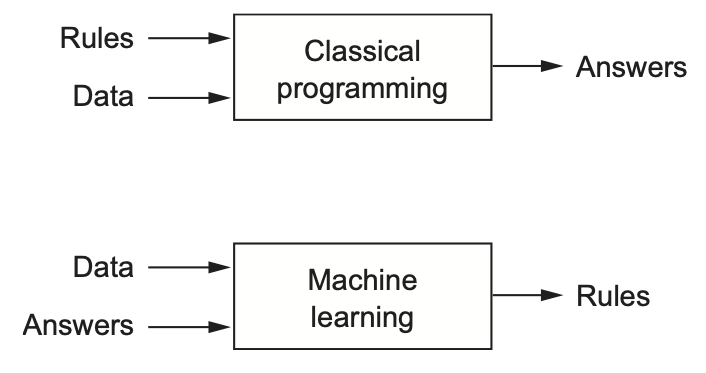
\includegraphics[width=0.8\textwidth]{figs/fig1_2_chollet.png}
\end{figure}

\end{frame}


\begin{frame}{Statistics and Machine Learning}

\begin{figure}[h]
\caption{Regression vs. Pure Predictions (Efron, 2020, Table 5)}
\centering
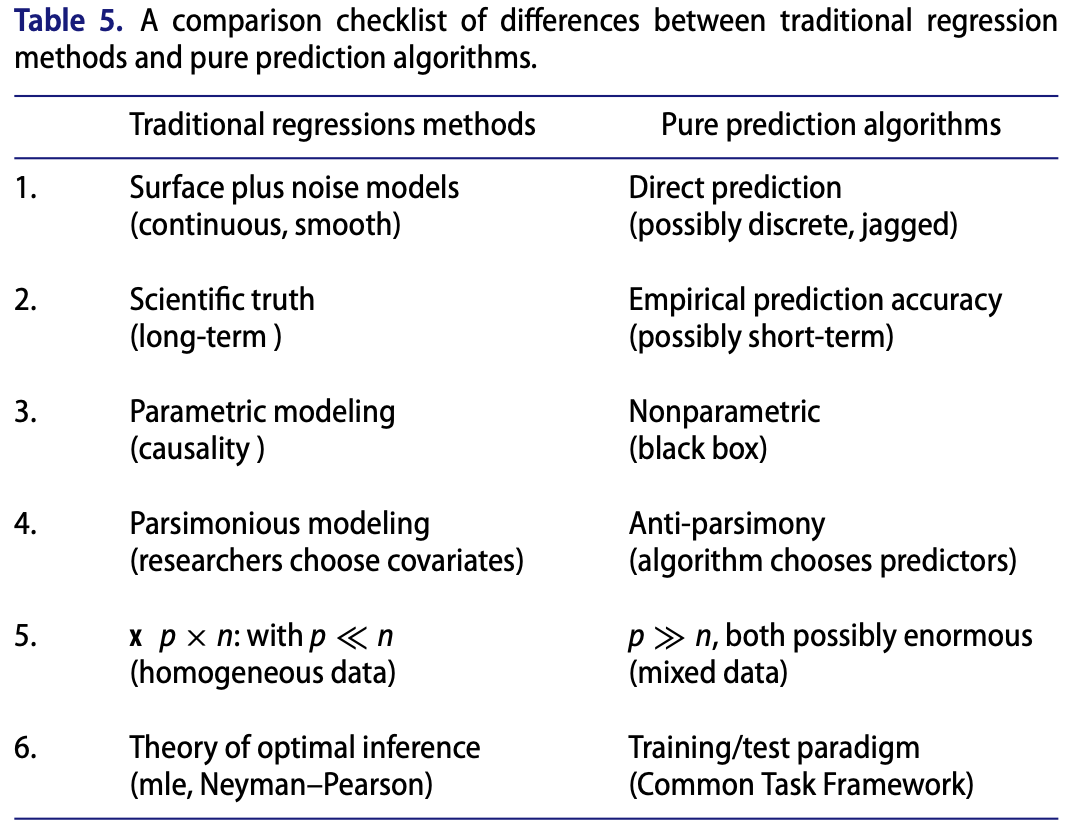
\includegraphics[width=0.8\textwidth]{figs/table5.png}
\end{figure}

\end{frame}


\begin{frame}{Different flavors of ML}

\begin{itemize}
\item Supervised learning
\item Unsupervised learning
\begin{itemize}
\item Self-(un)supervised learning
\end{itemize}
\item Reinforcement learning
\end{itemize}

\end{frame}


\begin{frame}<handout:0>{Questions?}
Questions?
\end{frame}

%%%%%%%%%%%%%%%%%%%%%%%%%%%%%%%%%%%%%%%%%%%%%%%%%%%%%%%%%%%%%%%%%%

\section{Course information}
\frame{\sectionpage}

\begin{frame}{Course information}
The aims of this course are that you should:\\[3mm]\pause
\begin{enumerate}
\item get a good knowledge of a large number of machine learning models,
\item become able to use methods for evaluating and improving predictive models,
\item become able to handle big data,
\item become able to train and use machine learning models in R,
\item become able to train and use neural networks using Keras/TensorFlow.
\item become able to describe and discuss ethical aspects of big data and black box-models,
\end{enumerate}

\end{frame}


\begin{frame}{Course Outline}
Two main parts:
\begin{itemize}
\item Core Content (8 blocks):
\begin{itemize}
\item Supervised learning (5 blocks)
\item Unsupervised learning (2 blocks)
\item Reinforcement learning (1 block)
\end{itemize}
\item Mini-project on a supervised project (2-3 students)\pause
\end{itemize}
Exact dates and details; see the course page.
\end{frame}

\begin{frame}{Core Content}

\begin{itemize}
\item Two lectures/computer labs (approx. 4h)
\item Online video material and reading assignments (approx. 4-6h, 50-90 pages a week)
\item \emph{Note!} There might be some overlap between reading instructions.
\item An individual computer assignment (approx. 12-16h). Deadline Sundays 23.59.\pause
\item Recommended workflow for each block
\begin{itemize}
\item Watch the videos (although, optional)
\item Do the reading assignments
\item Do the computer assignment
\end{itemize}
\end{itemize}

\end{frame}


\begin{frame}{Computer Assignments}

\begin{enumerate}
\item Main part of the course\\Learning by doing
\item Machine learning = Statistics + Computer Science\\Hence a lot of programming\pause
\item Both implementation of core components and state-of-the-art methods\pause
\item \emph{Warning!} There might be bugs in the assignments!\pause
\item All labs can be turned in a second time. Deadline 17th of January.
\end{enumerate}

\end{frame}

\begin{frame}{Mini-project}

\begin{itemize}
\item See project instructions on webpage for details.\pause
\item Supervised problem of choice on real data.
\item 2-3 students.\pause
\item Supply a half-page project proposal of data and problem at the end of block 6.\pause
\item Project will last two weeks (half time) - but start earlier.
\item Approximate 40 hours of work \emph{per student}.\pause
\item The project should result in a 4 page report (PDF) using the ICML LaTeX template.
\item Project oral presentation (10-15 minutes)\pause
\item Each student will review one other project:
\begin{enumerate}
\item Write a 1-2 page review of the report.
\item Discuss at the oral presentations.
\end{enumerate}
\end{itemize}
\end{frame}


\begin{frame}{Practicalities}

\begin{itemize}
\item Course page: Github -- please do a PR if something is wrong!\pause
\item Communication: Course Slack\pause
\item Acknowledgements: M{\aa}ns Thulin, Josef Wilzén, Anders Eklund\pause
\item Schedule: Time Edit/Studium
\item Assignments: Studium\pause
\item Literature
\begin{itemize}
\item Hastie, Tibshirani \& Friedman (2009). \emph{Elements of Statistical Learning}. Springer. Available at\\\texttt{https://web.stanford.edu/$\sim$hastie/ElemStatLearn/}
\item Chollet \& Allaire (2018). \emph{Deep Learning with R}. Manning. Available for reading at\\\texttt{https://www.manning.com/books/deep-learning-\\with-r}
\item Goodfellow, Bengio \& Courville (2017). \emph{Deep Learning}. Available at \\\texttt{https://www.deeplearningbook.org/}
\item Additional articles, tuturials, videos etc. posted on course (github) homepage
\end{itemize}
\end{itemize}

\end{frame}

\begin{frame}{Examination}

\begin{enumerate}
\item To pass (G): All labs, mini-project, and project review need to be passed\pause
\item To pass with distinction (VG): 7/10 VG points\pause
\item Each assignment has an extra (VG) task worth 1 VG point.\pause
\item The mini-project is worth 2 VG-points (if it is passed with distinction).
\end{enumerate}

\end{frame}

\begin{frame}<handout:0>{Questions?}
Questions?
\end{frame}

%%%%%%%%%%%%%%%%%%%%%%%%%%%%%%%%%%%%%%%%%%%%%%%%%%%%%%%%%%%%%%%%%%

\section{Introduction to Supervised Learning}
\frame{\sectionpage}

\begin{frame}{Supervised learning}

\begin{figure}[h]
\caption{Relationship between appartment size and price (\href{https://www.data-to-viz.com/story/TwoNum.html}{source})}
\centering
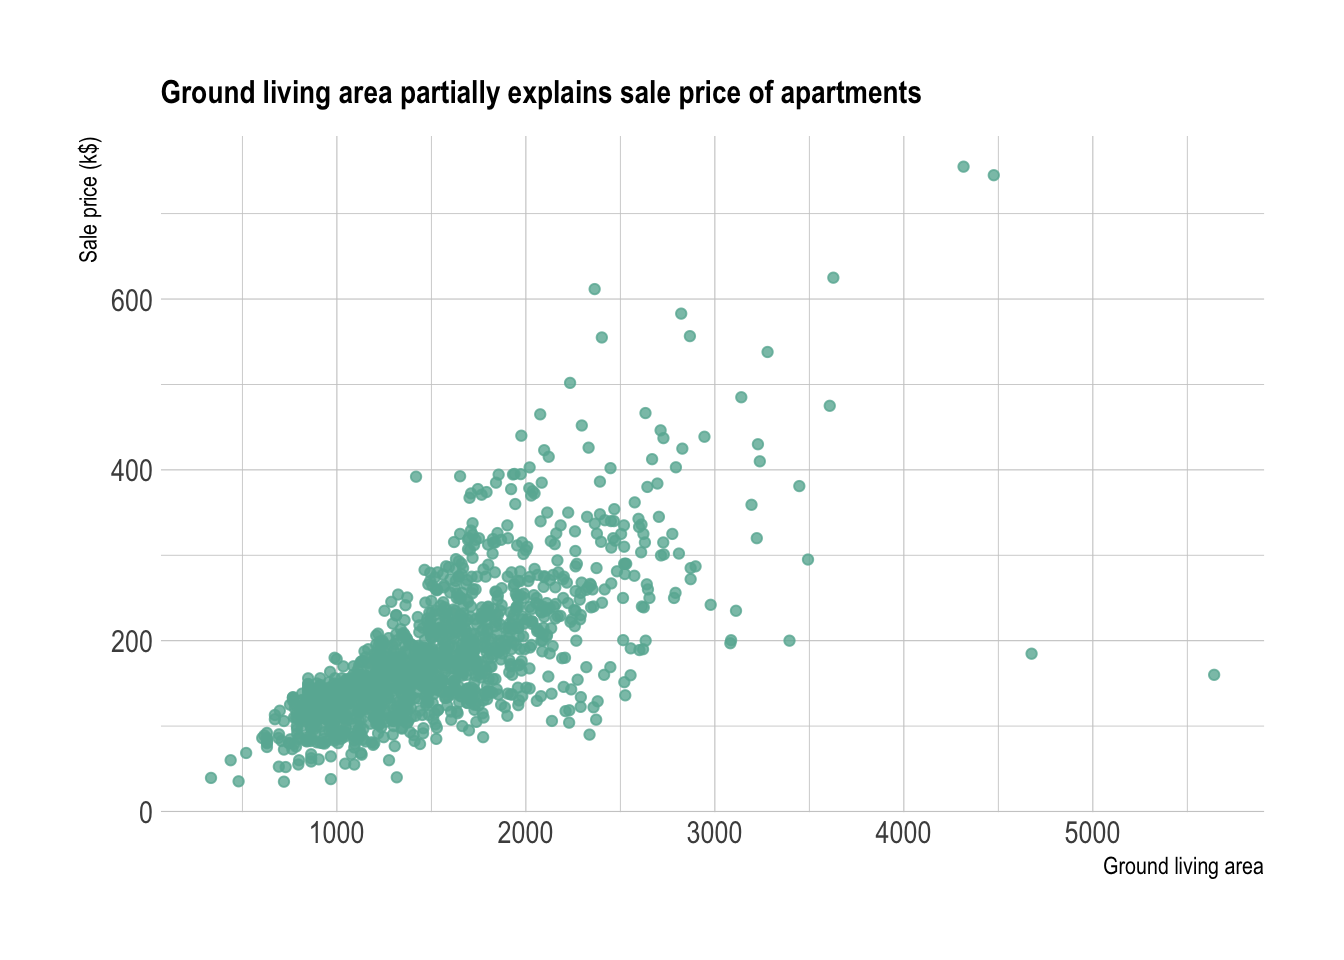
\includegraphics[width=0.8\textwidth]{figs/scatter_apartment.png}
\end{figure}

\emph{Problem}: We want to predict the price of a new apartment.

\end{frame}



\begin{frame}{Supervised learning}

\begin{itemize}
\item General problem: We have \emph{training} data
\[
\mathbf{d} = \{(y_i, \mathbf{x}_i), i = 1, ..., n\} \,.
\]
\item $\mathbf{x}_i = $ features/input/predictors/features/independent variables
\item $y_i = $ labels/output/dependent variable
\item We want to \emph{learn} a function $\hat{y} = f(x_{new})$ with as good performance as possible.\pause
\item Regression problems: $y_i \in \mathbb{R}$
\item Classification problems: $y_i \in {a,b,c,...}$ where $a,b,c ...$ are discrete classes.
\end{itemize}

\end{frame}



\begin{frame}{Example of supervised problems}

%[Take images - Ask are the classification problems or nor what is the features]

\begin{itemize}
\item Is this e-mail message spam (1) or not (0)?\pause
%\item Sequence to sequence (NLP) - machine translation?
\item Image recognition/classification\pause
\item Image object traction (position in a video)\pause
\item Will this patient recover from their illness or not?\pause
\item Does this fingerprint belong to an employee or not?\pause
\item Does this customer have stable finances or not?\pause
\item Face recognition\pause
\item Is this tumour malign (1) or not (0)?\pause
\end{itemize}

\end{frame}


\subsection{Example: Logistic regression}

\begin{frame}{Logistic regression and classification}
When the $y_i$ in a regression problem is binary (or more generally, categorical), it becomes a {\color{uured}classification problem}.\\[3mm]\pause
The question that the model tries to answer is: does this observation belong to class 0 or class 1?\\[3mm]\pause

Logistic regression is a workhorse in classification problems.


\end{frame}




\begin{frame}{Logistic regression}
When analysing binary data $y_1,\ldots,y_N$, we usually assume that the $Y_i$ follow binomial (or Bernoulli) distributions.\\[3mm ]\pause
Assume that $Y_1,\ldots,Y_N$ are independent with $Y_i \sim Bernoulli(\pi_i)$.\\[3mm ]\pause
$Y_i \in {0,1}$ with success probability $\pi_i$ and $\mu_i=E(Y_i)=\pi_i$.\\[3mm ]\pause
\begin{itemize}
\item The natural parameter of the binomial distribution is $$g(\pi_i)=\log\Big(\frac{\pi_i}{1-\pi_i}\Big),$$
called the {\color{uured}logit} or {\color{uured}log odds}.\\[3mm ]\pause
\item A GLM using this link function is called {\color{uured}logistic regression}, but other link functions are also often used in practice.\\[3mm]
\end{itemize}
\end{frame}


\begin{frame}{Logistic regression}
There are two equivalent formulas for {\color{uured}logistic regression}:
$$\log\Big(\frac{\pi_i}{1-\pi_i}\Big)=\beta_0+\beta_1 x_{i1}+\beta_2 x_{i2}+\cdots+\beta_p x_{ip},\qquad i=1,\ldots,N$$
and
$$\pi_i=\frac{\exp\Big(\beta_0+\sum_{j=1}^p\beta_jx_{ij}\Big)}{1+\exp\Big(\beta_0+\sum_{j=1}^p\beta_jx_{ij}\Big)}.$$
\end{frame}


\begin{frame}{Logistic regression: Prediction}
\begin{itemize}
\item We \emph{train} a logistic regression model using MLE using the training data.
\item Our estimation/traing output the MLE $\hat{\theta}$
\item We the compute $\hat{p}_i = g^{-1}(\hat{\theta} x_{new})$ a for a new observation
\item We use a {\color{uured} decision rule} to predict value 0 or 1:
\[
    \hat{y}_i(\hat{p}_i)=
\begin{cases}
    1,& \text{if } \hat{p}_i \geq 0.5\\
    0,              & \text{otherwise}
\end{cases}
\]
\end{itemize}
\end{frame}



\begin{frame}{Logistic regression: Example}


\begin{figure}[h]
\caption{Decision boundry with two covariates (Hastie et al, 2009, Figure 2.1) }
\centering
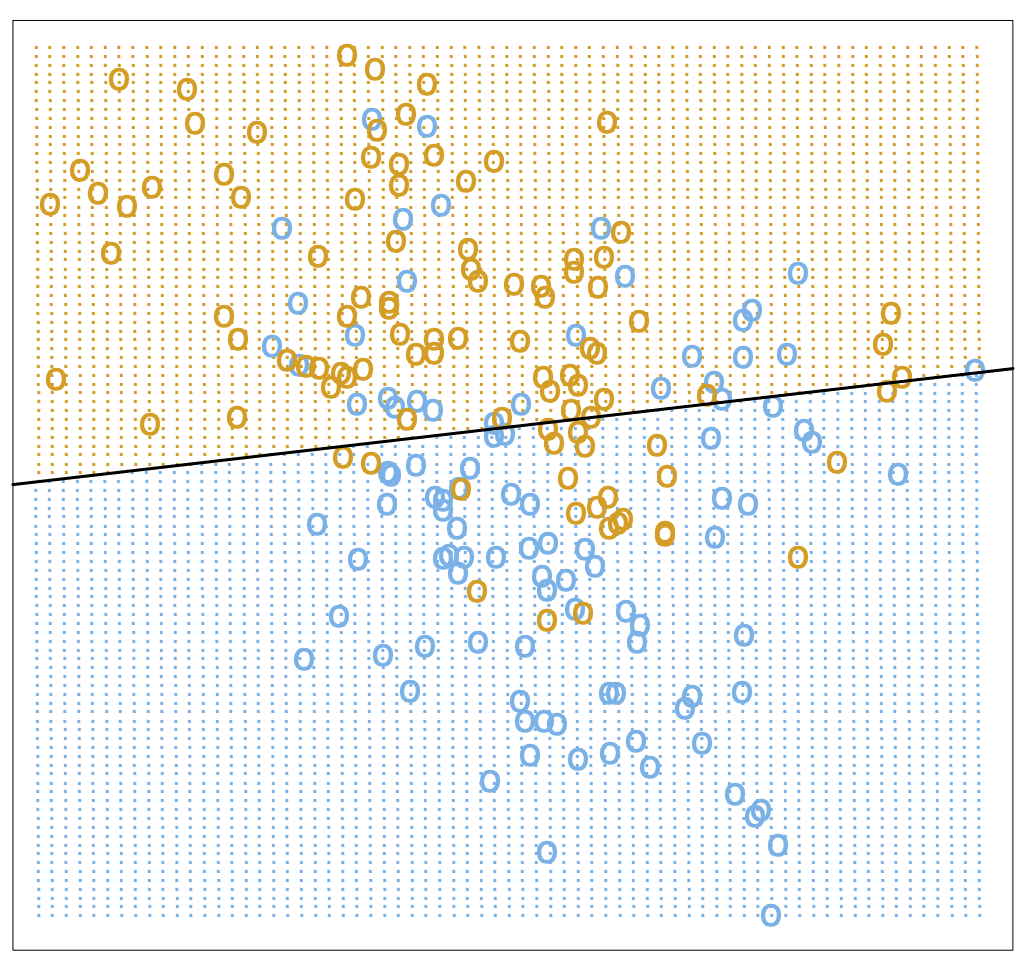
\includegraphics[width=0.7\textwidth]{figs/decision_fig_2_1.png}
\end{figure}

\end{frame}




\begin{frame}{An example: Spam and Ham}

\begin{columns}
	\begin{column}{0.47\textwidth}
		\textbf{E-mail Spam}\\
An e-mail provider what to help classify e-mails as spam (1) or ham (0). They have many previous e-mails that customers have already classified as spam, and e-mails people have responded (ham). They want to predict if a new, unseen e-mail is spam or ham.
	\end{column}
	\begin{column}{0.5\textwidth}
		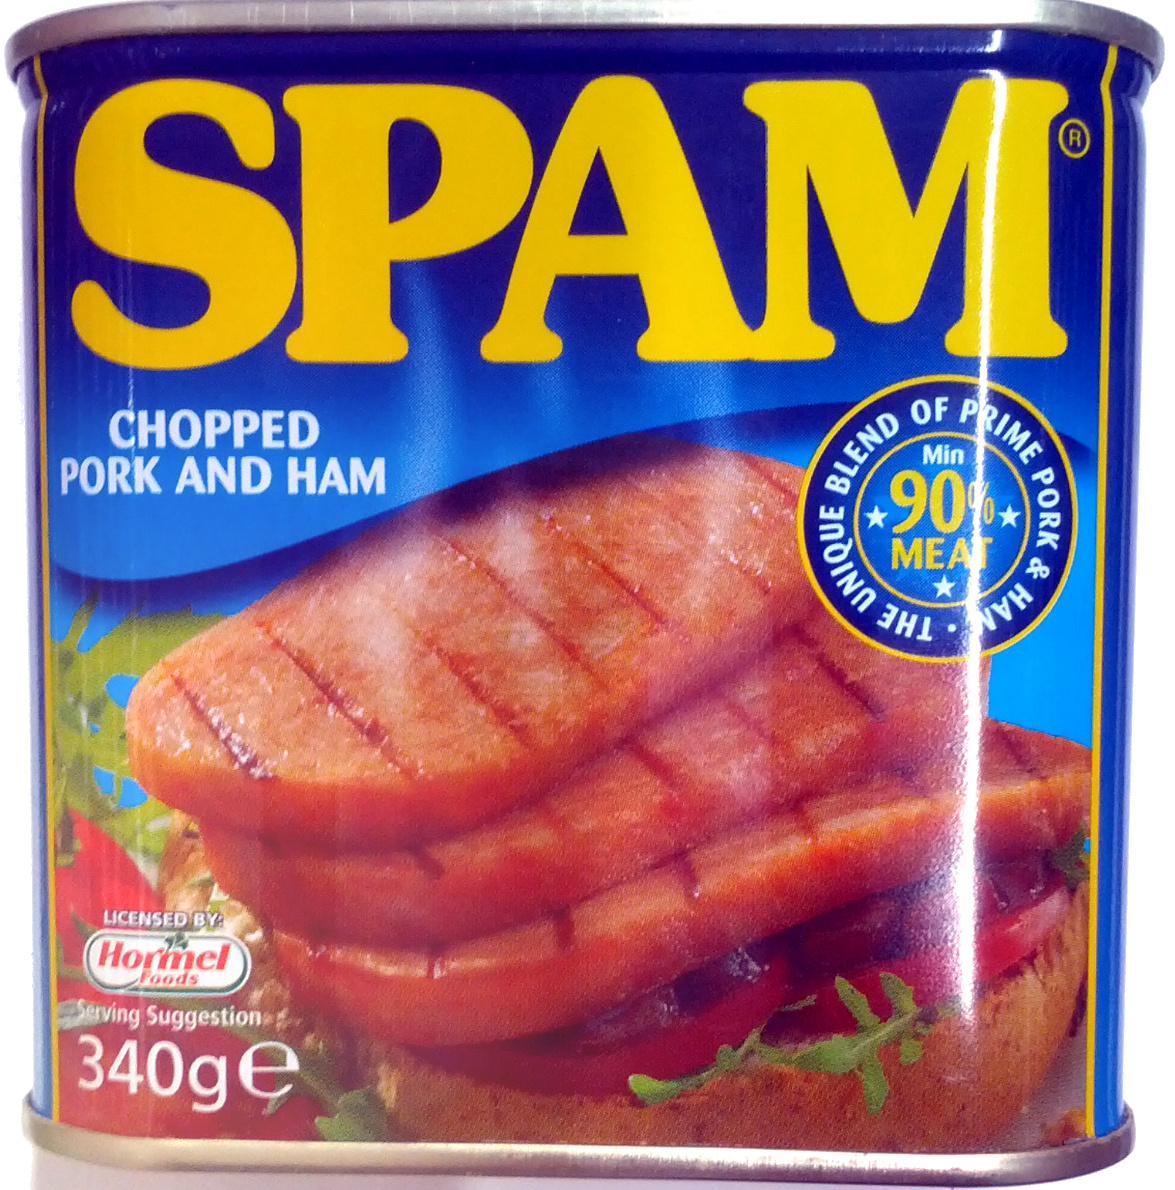
\includegraphics[width=\textwidth]{figs/spam.jpg}
%		(CC BY-SA 3.0)
	\end{column}
\end{columns}
\end{frame}


\begin{frame}<handout:0>{Questions?}

Questions?

\end{frame}

%%%%%%%%%%%%%%%%%%%%%%%%%%%%%%%%%%%%%%%%%%%%%%%%%%%%%%%%%%%%%%%%%%


\section{Optimization Algorithms for Machine Learning}
\frame{\sectionpage}

\begin{frame}{Training of ML algorithms}

\begin{enumerate}
\item Training is usually done by minimizing the objective/loss/cost function $L(\theta)$ for $\theta \in \mathbf{R}^P$.
\item Example: Logistic regression, here we can use the {\color{uured} negative} log-likelihood as loss function:
\[
L(\theta, \mathbf{y}, \mathbf{X}) = - \log \prod^N_{i=1} p_i^{y_i} (1 - p_i)^{1-y_i} \,,
\]
where
\[
\log \frac{p_i}{1-p_i} = \mathbf{x}_i \theta  \,,
\]\pause
\item In Machine Learning: $P$ and $N$ might be very large...
\end{enumerate}


\end{frame}



\begin{frame}{Gradient Decent}

\begin{enumerate}
\item The workhorse of Machine Learning
\[
\theta_t = \theta_{t-1} - \eta \nabla L(\theta_{t-1}, \mathbf{X}, \mathbf{y})\,,
\]
% the minus sign we go in the direction of steepest gradient - going down
where
\[
\nabla f(p)=\begin{bmatrix}{\frac {\partial f}{\partial x_{1}}}(p)\\\vdots \\{\frac {\partial f}{\partial x_{n}}}(p)\end{bmatrix}
\]
\item $L(\theta)$ needs to be differentiable
\end{enumerate}

\end{frame}


\begin{frame}{Gradient Descent Analogy}

\begin{figure}[h]
\caption{Gradient Descent Analogy (\href{https://en.wikipedia.org/wiki/Gradient_descent}{source})}
\centering
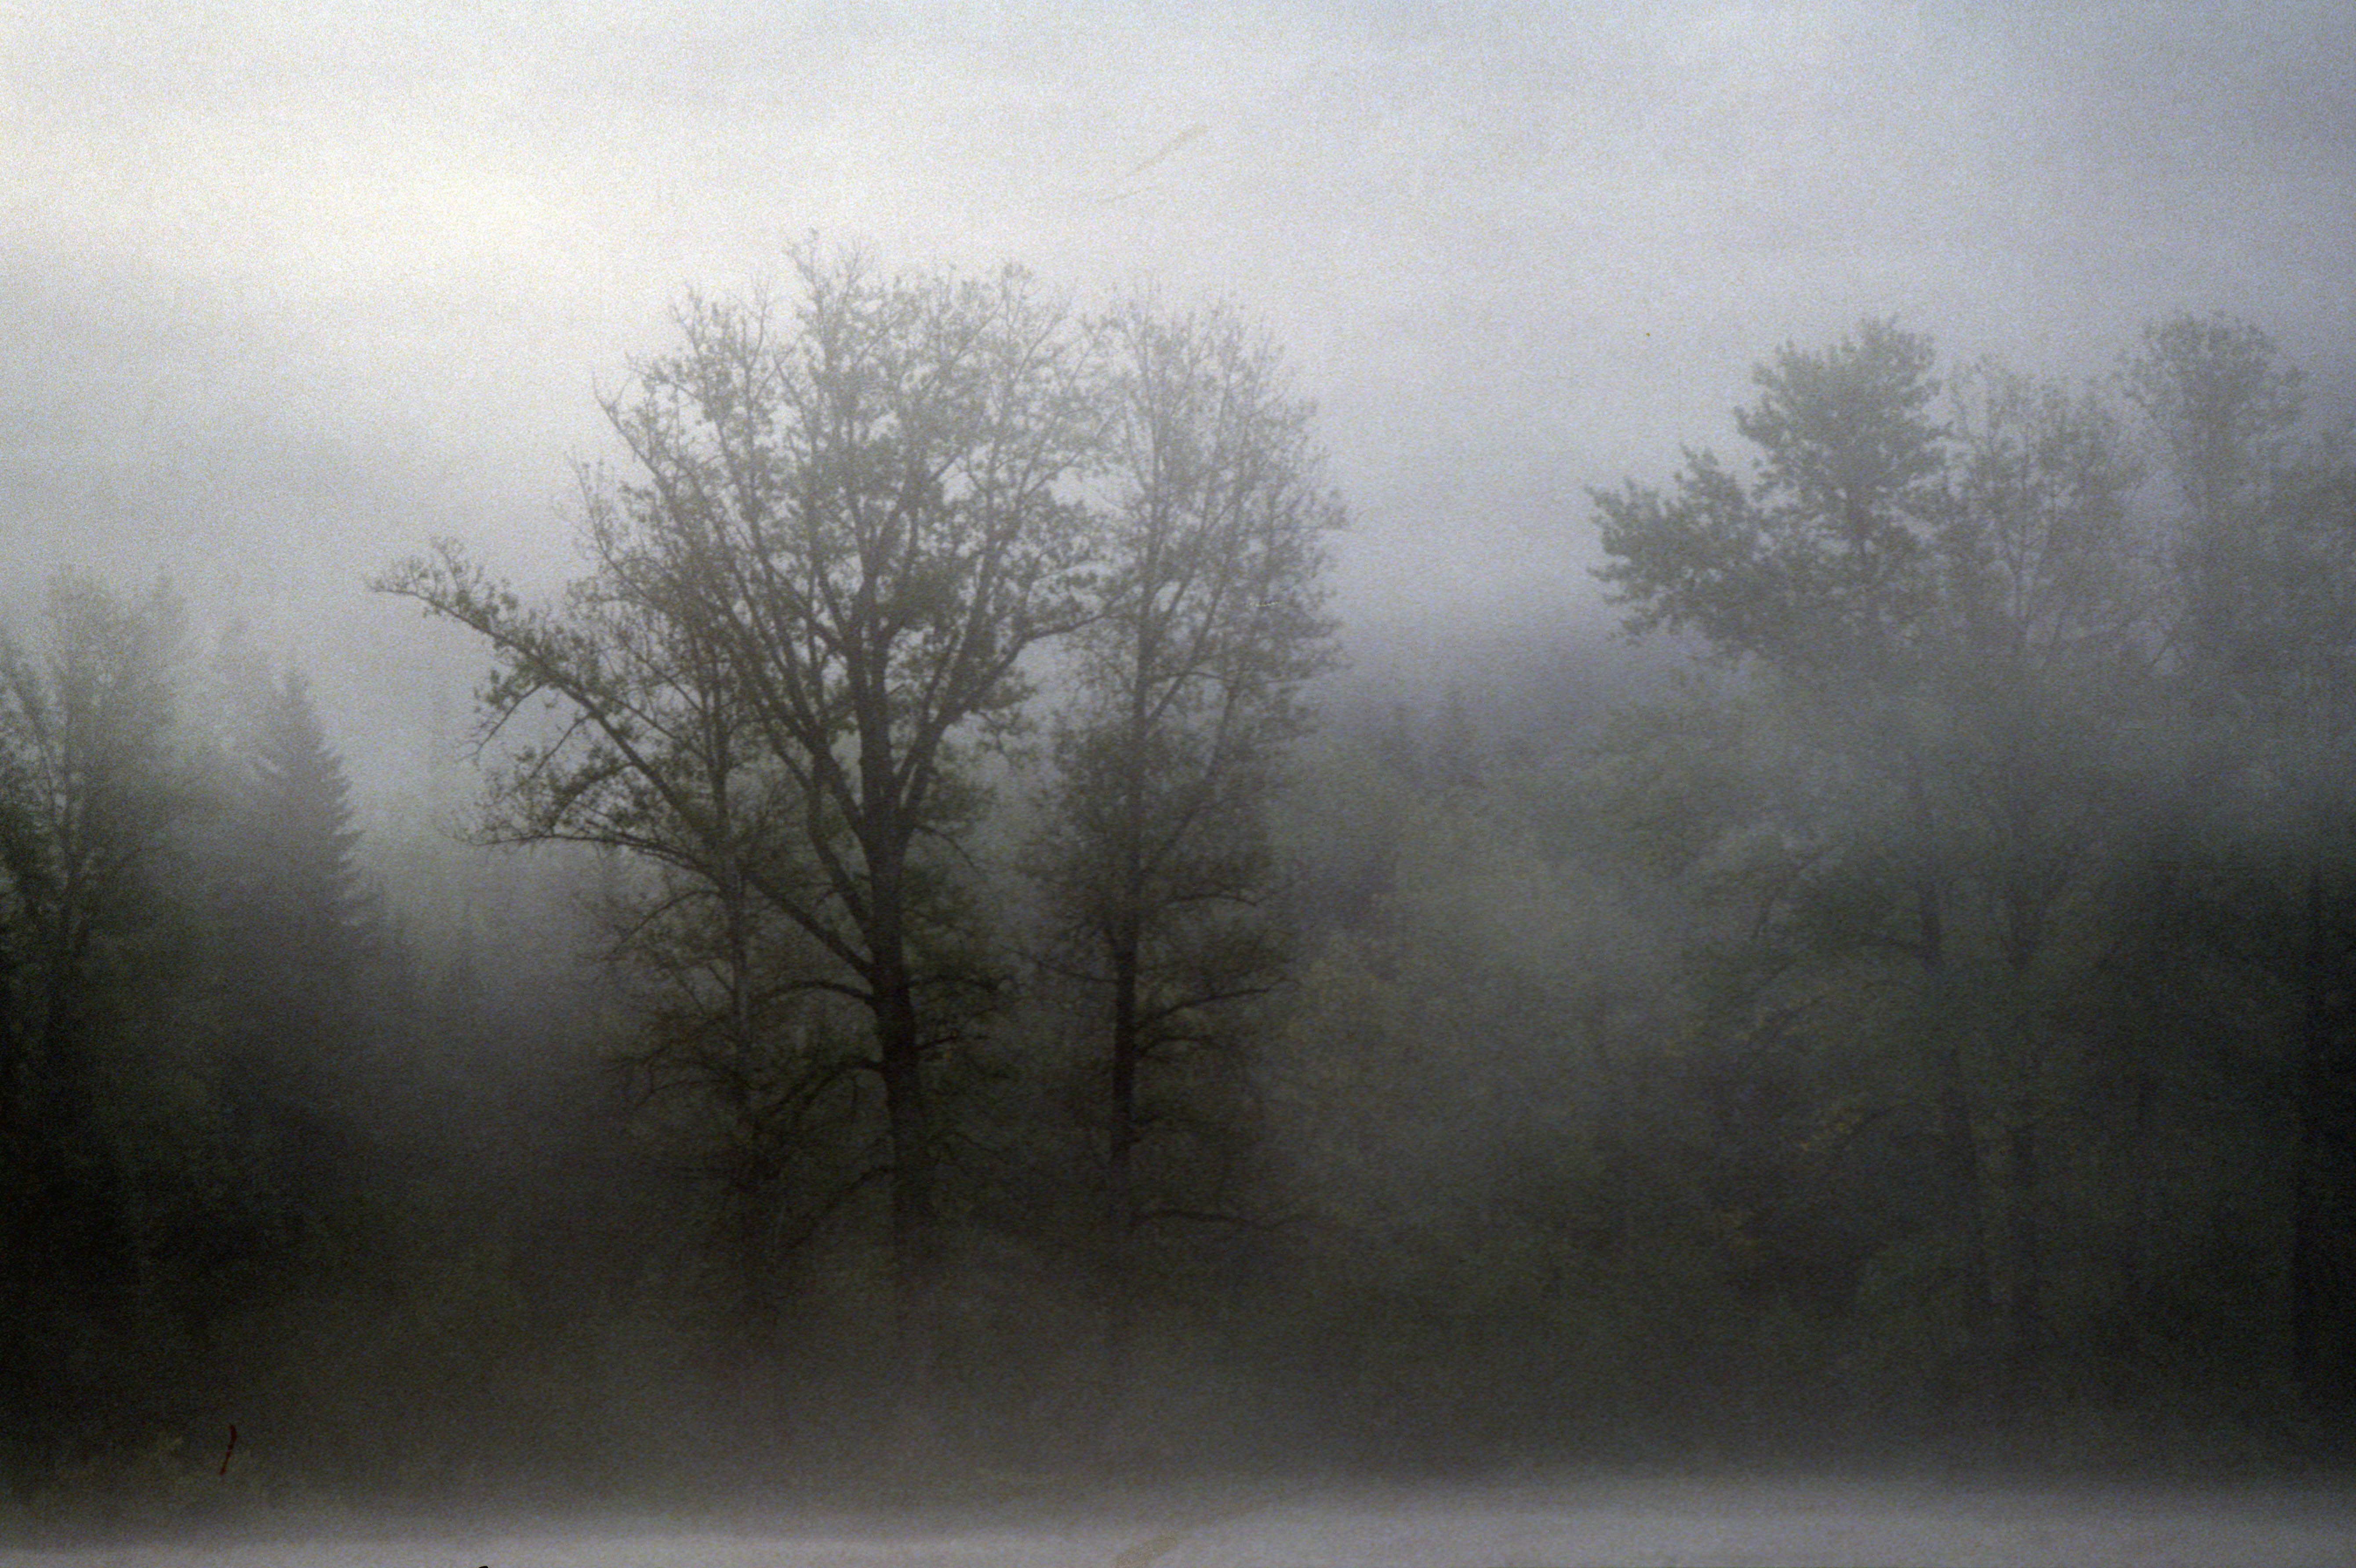
\includegraphics[width=0.8\textwidth]{figs/Okanogan-Wenatchee_National_Forest_morning_fog_shrouds_trees.jpg}
\end{figure}


\end{frame}



\begin{frame}{Gradient Descent (cont.)}

\begin{figure}[h]
\caption{Gradient Descent (\href{https://en.wikipedia.org/wiki/Gradient_descent}{source})}
\centering
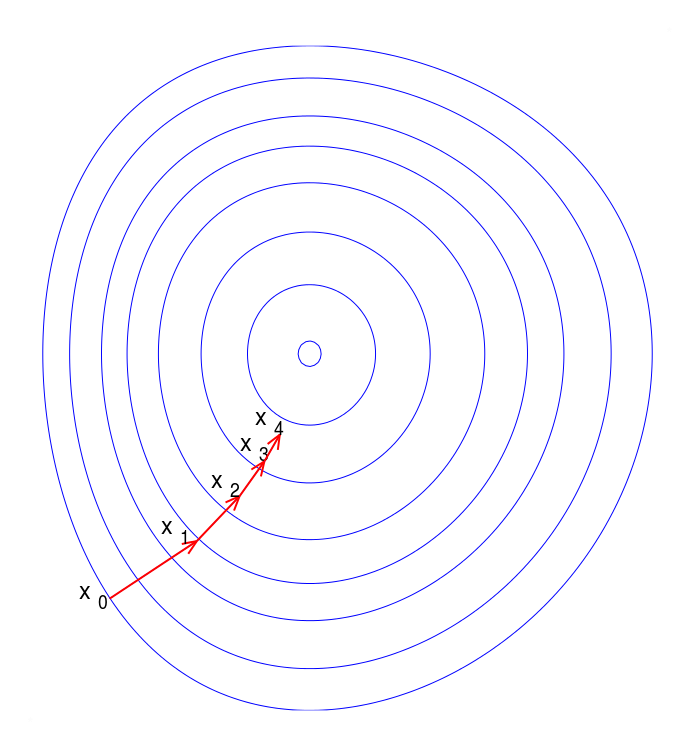
\includegraphics[width=0.7\textwidth]{figs/GD.png}
\end{figure}

\end{frame}




\begin{frame}{Why Gradient Descent?}


\begin{itemize}
\item Gradient Descent is a poor algorithm \\ (Newtons method, Iteratively Reweighted Least Squares are 'better')
\item So why is gradient descent relevant?\pause
\item The two benefits with Gradient Descent:
\begin{enumerate}
\item Only uses the gradient---scales to large $P$
\item Can scale to large data with Stochastic Gradient Descent---scales to large $N$
\end{enumerate}
\end{itemize}

\end{frame}


\begin{frame}{Stochastic Gradient Descent}


\begin{itemize}
\item Many loss functions (and gradients) are a sum over $N$ observations.
\item We can estimate $\nabla L(\theta, X_{i}, y_{i})$ by choosing a random observation (with index $i$)
\[
E(\nabla L(\theta, X_{i}, y_{i})) = \frac{1}{Z} \nabla L(\theta, \mathbf{X}, \mathbf{y})\,,
\]
for some constant $Z$.
\item Think survey sampling -- we want to estimate a total.
\item This give us the following algorithm:
\[
\theta_t = \theta_{t-1} - \eta_t \hat{\nabla} L(\theta_{t-1}, X_{i}, y_{i})\,,
\]
where $i$ is random sampled index.
\item \emph{Note!} \\We need to have an unbiased estimator for $\nabla L(\theta, \mathbf{X}, \mathbf{y})$
\item Epochs vs. Iterations
\end{itemize}


\end{frame}


\begin{frame}{Stochastic Gradient Descent}


\begin{itemize}
\item Learning rate $\eta_t$ is important
\item We need to reduce $\eta_t$ over time
\item Will it converge to an optimum?\pause
\item Robbins–Monro (1951) conditions:
\begin{enumerate}
\item $\eta_t \geq 0$ $\forall t \geq 0$
\item $\sum^\infty_t \eta_t = \infty$
\item $\sum^\infty_t \eta_t^2 < \infty$
\end{enumerate}
\end{itemize}

\end{frame}


\begin{frame}{Mini-batch gradient descent}

\begin{itemize}
\item Can we estimate the gradient better?\pause
\item We take a mini-batch of size $B$:
\[
\theta_t = \theta_{t-1} - \eta_t \nabla L(\theta, \mathbf{X}_{\mathcal(S)_i}, y_{\mathcal(S)_i})\,,
\]
where $\mathcal(S)_i$ is a set of random sample (without replacement) indices and $|\mathcal(S)_i| = B$.
\item $B$ is usually set to optimize hardware
\end{itemize}

\end{frame}


\begin{frame}{SGD with momentum}

\begin{itemize}
\item SGD can be slow to converge due to 'jumping' behaviour
\item Can improve behaviour using the velocity -- the rolling mean of gradients
\item Additional hyperparemeter $\alpha$ to control velocity
\[
v_t = \alpha v_{t-1} + \eta_t \hat{\nabla} L(\theta_{t-1}, X_{i}, y_{i})\,,
\]
\[
\theta_t = \theta_{t-1} - v_t,
\]

\end{itemize}


\end{frame}


\begin{frame}{SGD with momentum, Intuition}

\begin{figure}[h]
\caption{SGD with momentum, Intuition (CC)}
\centering
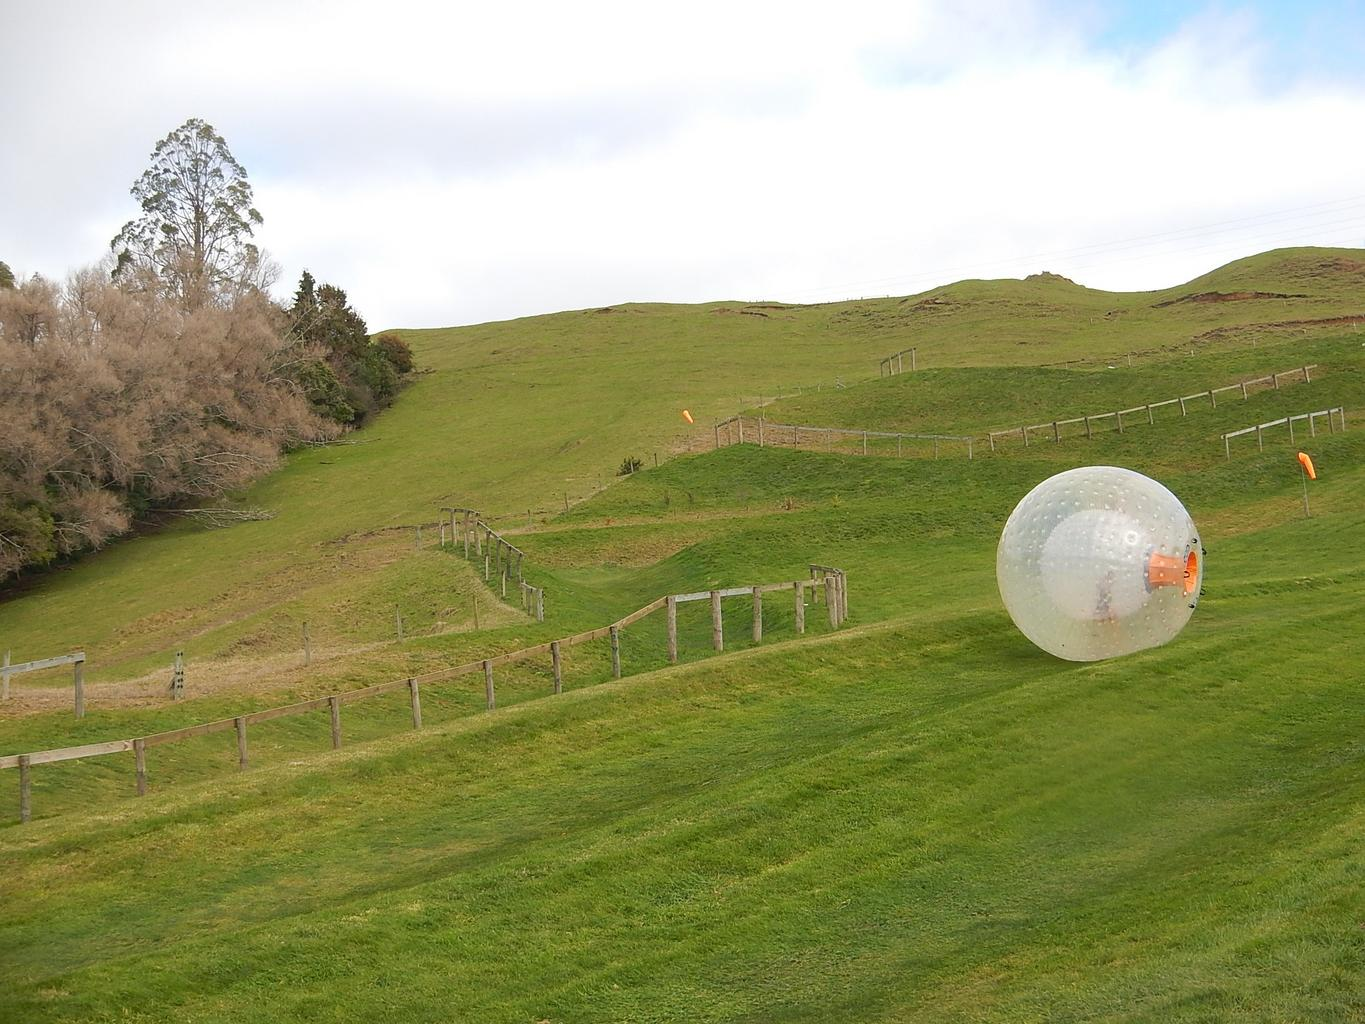
\includegraphics[width=0.9\textwidth]{figs/zorb}
\end{figure}

\end{frame}

\begin{frame}{SGD with momentum}

Example of SGD with momentum \href{https://distill.pub/2017/momentum/}{here}.

\end{frame}


\begin{frame}{Adam}

\begin{itemize}
\item Want the optimizer to adapt to the learning rate $\eta_t$ to individual parameters
\item Common approaches are
\begin{itemize}
\item RMSprop
\item Adaptive Moment Estimation (Adam)
\end{itemize}
\end{itemize}

\end{frame}





\end{document}



%%%%%%%%%%%%%%%%%%%%%%%%%%%%%%%%%%%%%%%%%%%%%%%%%%%%%%%%%%%%%%%%%%


\end{document}
